\newpage
\section{System Model and Problem Formulation}
\label{sec:system-model}

\subsection{Network Architecture}
\label{subsec:system-architecture}

The considered system is a three-tier LOCAL--EDGE--CLOUD computing continuum deployed over a \(200\,\mathrm{m} \times 200\,\mathrm{m}\) area. In PureEdgeSim, all end devices are instantiated as edge devices; task requests originate from these devices and may be executed locally, offloaded to one of several edge data centers, or forwarded to the cloud. \Figref{fig:network-topology} shows the simulation map used to visualize device placement, server locations, and coverage regions in the experimental area.

\begin{figure}[htbp]
    \centering
    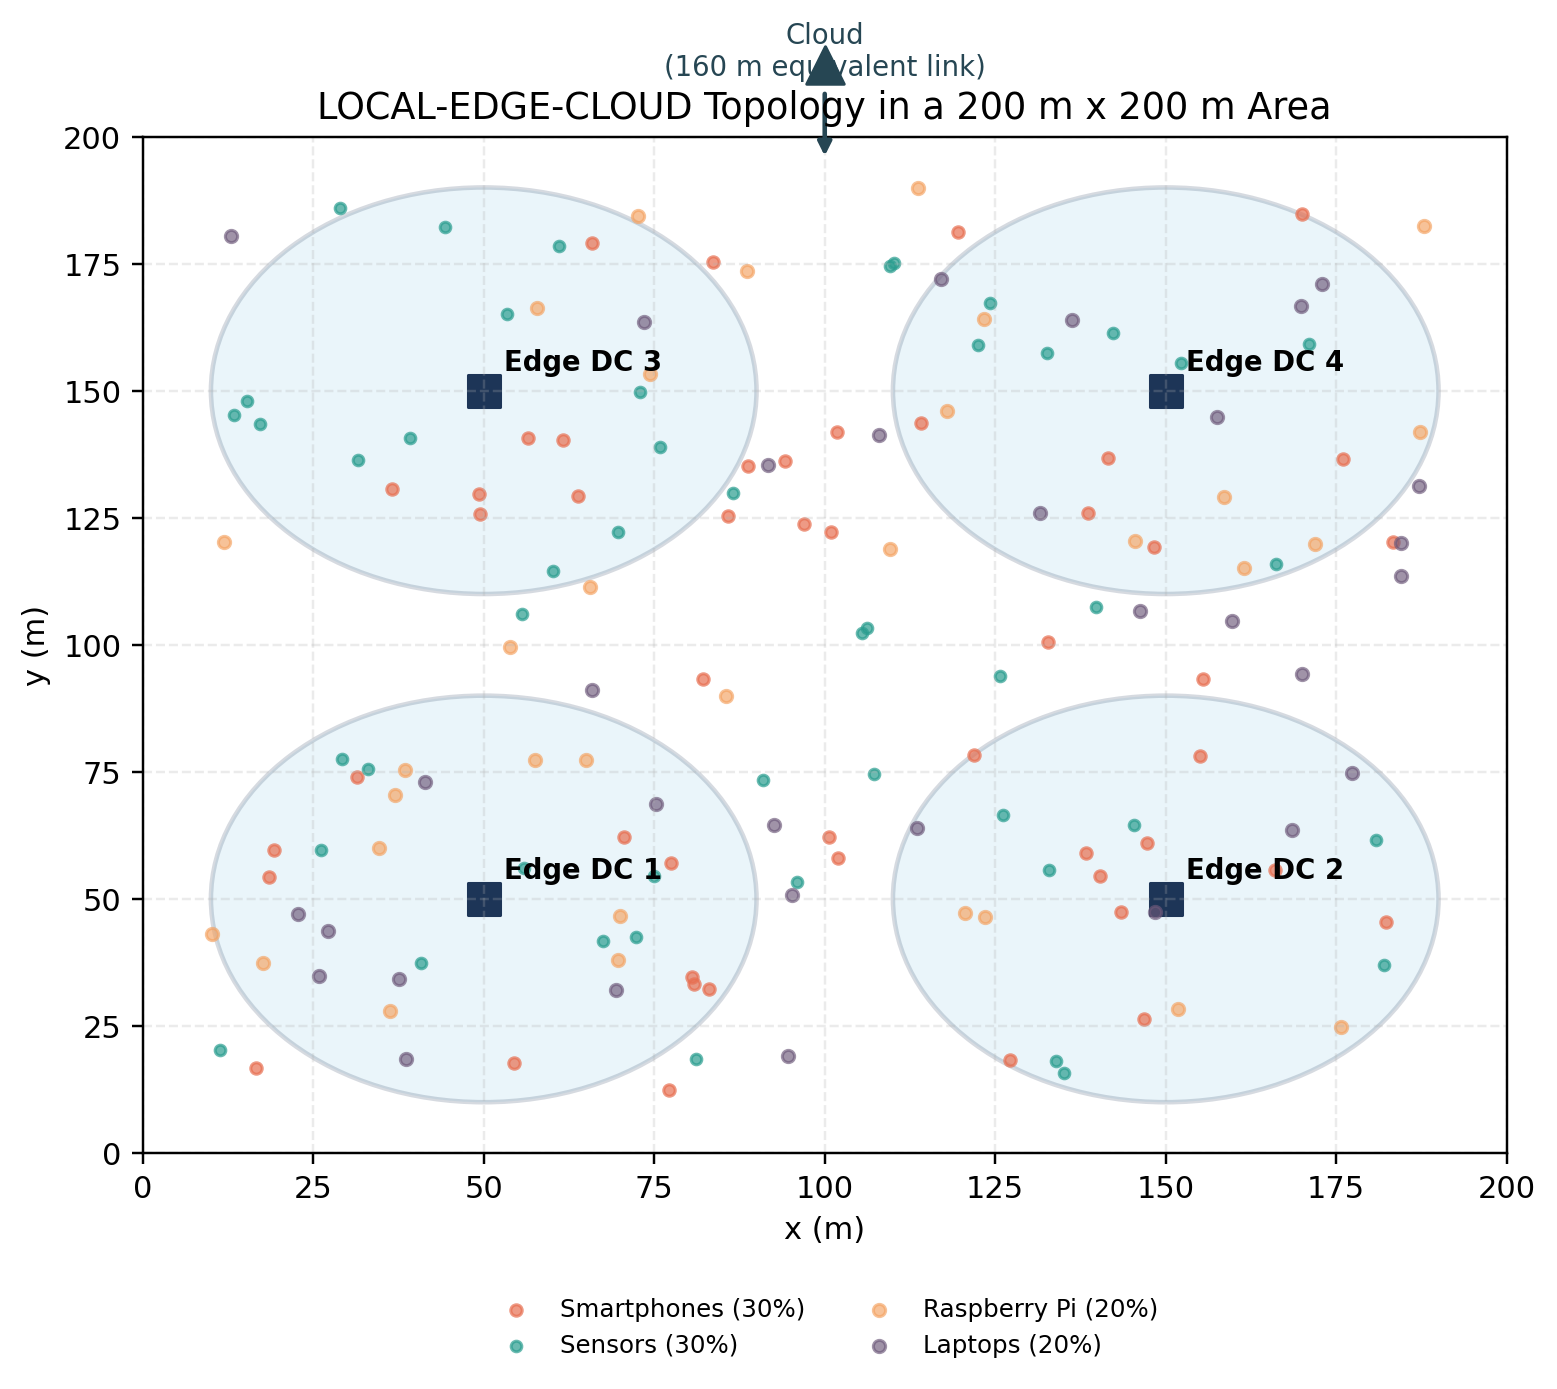
\includegraphics[width=0.92\textwidth]{figures/network_topology.png}
    \caption{Simulation map of the \(200\,\mathrm{m} \times 200\,\mathrm{m}\) deployment area, showing device states, server locations, and coverage regions.}
    \label{fig:network-topology}
\end{figure}

Four heterogeneous device classes are configured. Smartphones and sensors are the task-generating devices and therefore form the decision-making population in the RL formulation, whereas Raspberry Pi nodes and laptops serve as background devices that increase resource heterogeneity, spatial density, and wireless contention. The edge tier contains four identical edge data centers located at \((50,50)\), \((150,50)\), \((50,150)\), and \((150,150)\). Each edge data center has two hosts, and each host exposes eight virtual machines (VMs) with \(60{,}000\) MIPS per VM. The cloud tier contains one data center with two hosts and sixteen VMs in total, each providing \(150{,}000\) MIPS. Its communication-side abstraction is specified separately in \Secref{subsec:communication-model}.

\begin{table}[htbp]
    \centering
    \resizebox{\textwidth}{!}{%
    \begin{tabular}{p{0.23\linewidth}cccccc}
        \hline
        \textbf{Device type} & \textbf{Share} & \textbf{Task gen.} & \textbf{Mobility} & \textbf{CPU} & \textbf{RAM} & \textbf{Local VM} \\
        \hline
        Smartphone & 30\% & yes & \(1.4\,\mathrm{m/s}\) & \(20{,}000\) MIPS & 4 GB & 1 VM \\
        Raspberry Pi & 20\% & no & fixed & \(8{,}000\) MIPS & 4 GB & 1 VM \\
        Laptop & 20\% & no & fixed & \(60{,}000\) MIPS & 8 GB & 1 VM \\
        Sensor & 30\% & yes & fixed & no VM & 4 GB & none \\
        \hline
    \end{tabular}
    }
    \caption{Heterogeneous end-device configuration.}
    \label{tab:edge-device-config}
\end{table}

\begin{table}[htbp]
    \centering
    \small
    \renewcommand{\arraystretch}{1.18}
    \begin{tabularx}{0.96\textwidth}{>{\raggedright\arraybackslash}p{0.12\textwidth}>{\raggedright\arraybackslash}X>{\raggedright\arraybackslash}X>{\raggedright\arraybackslash}p{0.20\textwidth}}
        \hline
        \textbf{Tier} & \textbf{Deployment} & \textbf{Compute configuration} & \textbf{Communication note} \\
        \hline
        Edge DC & 4 edge data centers located at \((50,50)\), \((150,50)\), \((50,150)\), and \((150,150)\) & Each data center contains \(2\) hosts with \(8\) VMs per host, and each VM provides \(60{,}000\) MIPS & Wireless coverage radius: \(120\,\mathrm{m}\) \\
        Cloud & 1 remote cloud tier represented as an abstract backbone-connected node & \(2\) hosts with \(8\) VMs per host, and each VM provides \(150{,}000\) MIPS & PRB-side link abstraction is defined separately in \Secref{subsec:communication-model} \\
        \hline
    \end{tabularx}
    \caption{Edge-tier and cloud-tier server configuration.}
    \label{tab:server-config}
\end{table}

An important modeling detail is that sensor nodes do not host a local VM. Consequently, the local-execution option is infeasible for those devices and is masked out automatically during decision making.

\subsection{Task Model}
\label{subsec:task-model}

Three application classes are used to generate workloads with distinct latency and communication requirements. Their generation rates, latency deadlines, and workload sizes are specified in \texttt{applications.xml}. For each arriving task, the controller chooses an execution destination from the feasible set consisting of local execution, the reachable edge data centers, and the cloud.

\begin{table}[htbp]
    \centering
    \resizebox{\textwidth}{!}{%
    \begin{tabular}{p{0.28\linewidth}ccccc}
        \hline
        \textbf{Application} & \textbf{Rate (/min)} & \textbf{Share} & \textbf{Max delay (s)} & \textbf{Request size (KB)} & \textbf{Task length (MI)} \\
        \hline
        AUGMENTED\_REALITY & 25 & 20\% & 8 & 1500 & 80{,}000 \\
        E\_HEALTH & 20 & 25\% & 25 & 10{,}000 & 400{,}000 \\
        HEAVY\_COMP\_APP & 25 & 30\% & 12 & 50 & 120{,}000 \\
        \hline
    \end{tabular}
    }
    \caption{Application workload configuration and result sizes.}
    \label{tab:application-config}
\end{table}

The task lifecycle in PureEdgeSim proceeds through orchestration, transmission, execution, and result return events. At a high level, the event chain is
\begin{align*}
\texttt{SEND\_TO\_ORCH} \rightarrow \texttt{SEND\_TO\_DEST} \rightarrow \texttt{EXECUTE}
\rightarrow \texttt{TRANSFER\_RESULTS} \rightarrow \texttt{FINISHED}.
\end{align*}
Task failure occurs when the end-to-end latency exceeds the application deadline, communication becomes infeasible because of coverage or mobility constraints, or no valid execution resource can be allocated.

\subsection{Communication Model}
\label{subsec:communication-model}

Wireless communication is modeled at the PRB level. The total WLAN capacity is \(5000\,\mathrm{Mbps}\), discretized into \(5000\) PRB blocks. If a transfer is assigned \(b\) blocks, its effective bandwidth is
\begin{align}
BW = \frac{BW_{\mathrm{WLAN}}}{PRB_{\mathrm{total}}} \times b \times
\min \left(1.0, \left(\frac{d_0}{\max(d, d_0)}\right)^\alpha \right),
\label{eq:bandwidth-prb}
\end{align}
where \(d\) is the transmission distance, \(d_0 = 20\,\mathrm{m}\) is the reference distance, and \(\alpha = 0.5\) is the distance-attenuation exponent.

Two PRB allocation modes are supported. For RL-based algorithms, the selected PRB action is mapped to a fixed reservation before transmission begins. Under the default configuration, the per-task PRB cap is \(B_{\max} = 0.01 \times 5000 = 50\) blocks. The eight discrete actions correspond to
\begin{align*}
\rho \in \{0.02, 0.05, 0.10, 0.20, 0.40, 0.60, 0.80, 1.00\},
\end{align*}
and the requested reservation is computed as \(b = \max(1, \lfloor \rho B_{\max} \rfloor)\). The reserved blocks are released once the upload phase completes. 

For non-RL algorithms, the task does not request a fixed PRB quota, and the network model therefore handles the transfer through its dynamic allocation path. Before the transfer is admitted, the simulator checks whether the conflicting LAN activity still leaves enough unreserved PRBs to guarantee at least one block for the new transfer together with the already active dynamic transfers; otherwise, the task is rejected as a network failure. During each network update, the active transfers are partitioned into conflict components by breadth-first traversal over transfers that share a communication endpoint. Within each component, PRBs already reserved by fixed-allocation transfers are preserved, each dynamic transfer first receives one PRB block, and the remaining blocks are then distributed proportionally according to the weight \(1 + \texttt{lanPriorityBin}\), with any residual blocks assigned by descending fractional remainder.

If a fixed reservation would exceed the global PRB pool, the transfer is rejected and the corresponding task fails because of network infeasibility. In the PRB-based bandwidth model, any transfer involving the cloud is assigned a fixed equivalent distance of \(160\,\mathrm{m}\) through \texttt{CLOUD\_COVERAGE\_DISTANCE}. This constant is used to compute communication-side attenuation and PRB demand, so the cloud is penalized as a more remote destination without introducing a separate WAN model.

\subsection{Computation Model}
\label{subsec:computation-model}

All VMs use the \texttt{SPACE\_SHARED} scheduling policy. Let \(L\) denote the task length in million instructions and let \(M\) denote the MIPS capacity of the assigned VM. The nominal execution time is
\begin{align}
T_{\mathrm{exec}} = \frac{L}{M}.
\label{eq:exec-time}
\end{align}
In the actual scheduler, destination evaluation uses estimated finish time rather than only the nominal service time. The simulator approximates queueing pressure by scaling each VM's effective MIPS according to its current running-task count. The resulting finish-time estimate is used both in the destination features and in the fallback rule that resolves infeasible destination requests.

\subsection{Energy Model}
\label{subsec:energy-model}

Wireless transmission energy follows the simulator's radio model
\begin{align}
E_{\mathrm{tx}} = E_{\mathrm{elec}} \cdot bits + E_{\mathrm{amp}} \cdot bits \cdot d^n,
\label{eq:energy-model}
\end{align}
where \(E_{\mathrm{elec}} = 5 \times 10^{-8}\,\mathrm{J/bit}\), \(E_{\mathrm{amp}} = 10^{-11}\,\mathrm{J/bit/m^2}\) in the free-space regime, and \(E_{\mathrm{amp}} = 1.3 \times 10^{-15}\,\mathrm{J/bit/m^4}\) in the multipath regime. The simulator accumulates the resulting communication cost into the per-task total energy. It should be noted that this energy module uses a separate coarse distance approximation: transfers involving the cloud or an edge data center reuse the data-center communication range rather than the \(160\,\mathrm{m}\) cloud constant from the bandwidth model. To stabilize policy learning, the reward does not use raw energy directly; instead, the task energy is standardized online through exponential moving estimates of the mean and variance with smoothing factor \(\alpha = 0.01\).

\subsection{Problem Formulation}
\label{subsec:problem-formulation}

The scheduling objective is to jointly determine the execution destination and wireless-resource reservation for each task so as to improve deadline satisfaction while limiting energy consumption and PRB usage. Because decisions are made by many devices under partial observability and shared resource constraints, the problem is modeled as a cooperative Dec-POMDP
\begin{align*}
\mathcal{G} = \left\langle \mathcal{N}, \mathcal{S}, \{\mathcal{O}_i\}_{i \in \mathcal{N}},
\{\mathcal{A}_i\}_{i \in \mathcal{N}}, P, R \right\rangle .
\end{align*}

The agent set \(\mathcal{N}\) contains all task-generating devices, ordered by data-center identifier. Although decisions are emitted asynchronously as tasks arrive at the orchestrator, the agents are coupled through the same evolving compute queues, mobility conditions, and shared PRB pool. For agent \(i\), the local observation \(o_i \in \mathcal{O}_i\) contains a 13-dimensional device feature vector and an \(N_{\mathrm{dest}} \times 11\) destination-feature matrix. The candidate destinations are ordered as local execution first, followed by edge data centers sorted by identifier, and then cloud destinations. Under the reported topology, \(N_{\mathrm{dest}} = 6\). The base global state \(s \in \mathcal{S}\) is a 27-dimensional system summary; the MAPPO-specific critic augmentation used later in \Secref{sec:methodology} is built on top of this base state rather than replacing it.

The action of agent \(i\) at decision step \(t\) is
\begin{align*}
a_{i,t} = \left(a_{i,t}^{\mathrm{dest}}, a_{i,t}^{\mathrm{prb}}\right) \in
\mathcal{A}_i^{\mathrm{dest}} \times \mathcal{A}_i^{\mathrm{prb}},
\end{align*}
where \(a_{i,t}^{\mathrm{dest}}\) selects the execution destination and \(a_{i,t}^{\mathrm{prb}}\) selects one of the eight PRB bins. When local execution is chosen, no uplink reservation is needed and the PRB action is forced to zero.

Let \(\pi = \{\pi_i\}_{i \in \mathcal{N}}\) denote the decentralized device policies. For decision step \(t\), let \(F_t \in \{0,1\}\) be the task-failure indicator, let \(Z_t \in \{0,1\}\) indicate whether the requested destination is replaced by a feasible fallback, let \(\widetilde{L}_t\) denote the latency ratio, let \(\widetilde{E}_t\) denote the online-standardized energy term, and let \(\widetilde{B}_t\) denote the normalized PRB cost. A natural long-run system objective is to minimize the average weighted cost
\begin{align}
J(\pi) = \E_{\pi} \left[\frac{1}{T}\sum_{t=1}^{T}
\left(\lambda_f F_t + (1-F_t)\left(\lambda_l \widetilde{L}_t + \lambda_e \widetilde{E}_t
+ \lambda_b \widetilde{B}_t + \lambda_z Z_t\right)\right)\right].
\label{eq:policy-objective}
\end{align}
In the implemented simulator, policy learning uses the following shaped task-level reward:
\begin{align}
R_t =
\begin{cases}
-5.0, & \text{if the task fails},\\
5.0 - \widetilde{L}_t - 2.0\widetilde{E}_t - 1.5\widetilde{B}_t - 1.5 Z_t, & \text{if the task succeeds},
\end{cases}
\label{eq:implemented-reward}
\end{align}
This reward assigns a hard penalty to task failure and otherwise trades off latency, energy consumption, reserved PRBs, and fallback corrections. The corresponding decision process is subject to the practical constraints
\begin{align*}
a_{i,t}^{\mathrm{dest}} &\in \mathcal{D}_{i,t}^{\mathrm{feas}}, \\
0 \le b_{i,t} &\le B_{\max}, \\
\sum_{u \in \mathcal{U}_t^{\mathrm{fix}}} b_u &\le B_{\mathrm{tot}}, \\
T_t &\le D_t \quad \text{for a task to be counted as successful},
\end{align*}
where \(\mathcal{D}_{i,t}^{\mathrm{feas}}\) is the feasible destination set induced by coverage, VM availability, and network admission, \(b_{i,t}\) is the reserved PRB count mapped from the chosen bin, \(B_{\mathrm{tot}}\) is the total PRB budget, and \(D_t\) is the task deadline.

The transition kernel \(P\) is not derived analytically. Instead, state transitions are generated by the PureEdgeSim discrete-event engine, which jointly captures task arrivals, mobility, queueing, VM execution, and wireless contention. This simulator-defined dynamics is precisely the reason a reinforcement-learning formulation is preferable here to a closed-form optimization model.
